
\hspace{-1cm}
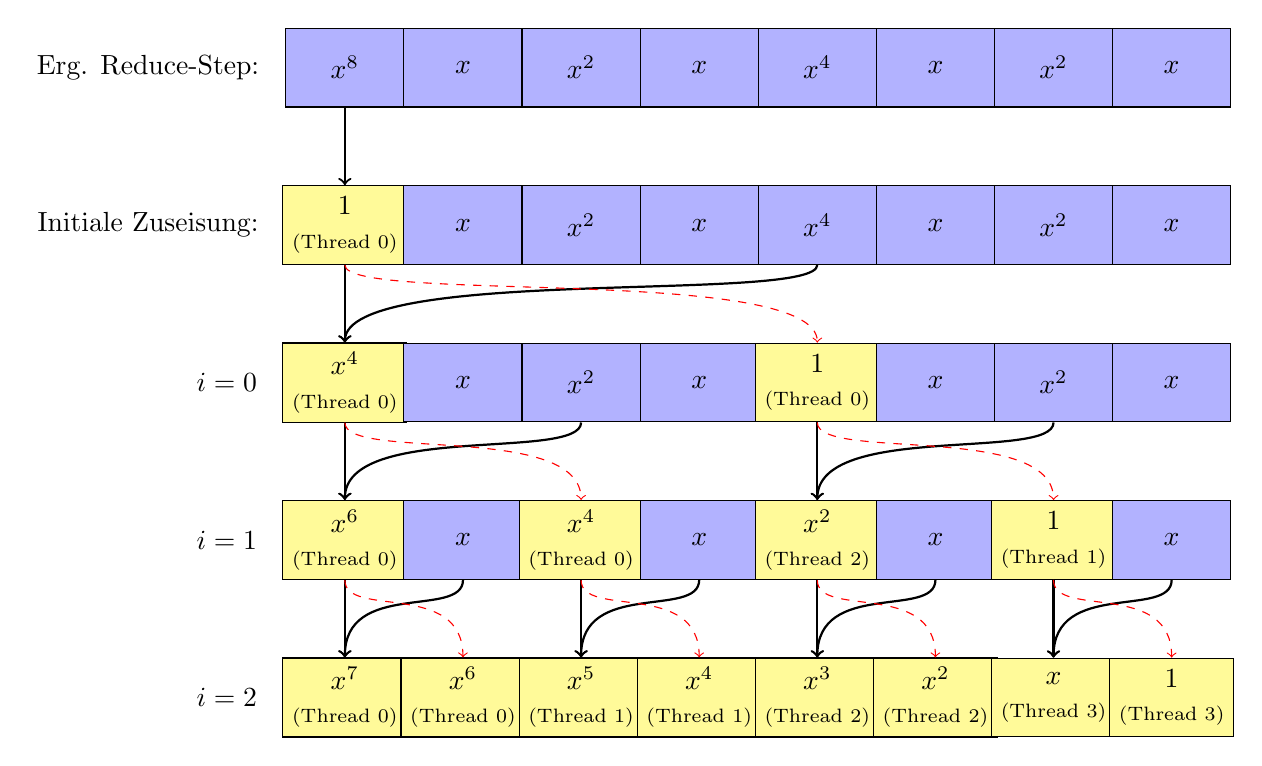
\begin{tikzpicture}[level/.style={sibling distance=60mm/#1}]

\def\HEIGHT{1}
\def\WIDTH{1.5}

% leaves
\node (rect) at (0*\WIDTH,10) [draw,minimum width=\WIDTH cm,minimum height=\HEIGHT cm, fill=blue!30] (a0) {$x^8$};
\node (rect) at (1*\WIDTH,10) [draw,minimum width=\WIDTH cm,minimum height=\HEIGHT cm, fill=blue!30] (a1) {$x$};
\node (rect) at (2*\WIDTH,10) [draw,minimum width=\WIDTH cm,minimum height=\HEIGHT cm, fill=blue!30] (a2) {$x^2$};
\node (rect) at (3*\WIDTH,10) [draw,minimum width=\WIDTH cm,minimum height=\HEIGHT cm, fill=blue!30] (a3) {$x$};
\node (rect) at (4*\WIDTH,10) [draw,minimum width=\WIDTH cm,minimum height=\HEIGHT cm, fill=blue!30] (a4) {$x^4$};
\node (rect) at (5*\WIDTH,10) [draw,minimum width=\WIDTH cm,minimum height=\HEIGHT cm, fill=blue!30] (a5) {$x$};
\node (rect) at (6*\WIDTH,10) [draw,minimum width=\WIDTH cm,minimum height=\HEIGHT cm, fill=blue!30] (a6) {$x^2$};
\node (rect) at (7*\WIDTH,10) [draw,minimum width=\WIDTH cm,minimum height=\HEIGHT cm, fill=blue!30] (a7) {$x$};

\node (rect) at (0*\WIDTH,8) [draw,minimum width=\WIDTH cm,minimum height=\HEIGHT cm, fill=yellow!40, align=center] (b0) {$1$\\\scriptsize{(Thread 0)}};
\node (rect) at (1*\WIDTH,8) [draw,minimum width=\WIDTH cm,minimum height=\HEIGHT cm, fill=blue!30] (b1) {$x$};
\node (rect) at (2*\WIDTH,8) [draw,minimum width=\WIDTH cm,minimum height=\HEIGHT cm, fill=blue!30] (b2) {$x^2$};
\node (rect) at (3*\WIDTH,8) [draw,minimum width=\WIDTH cm,minimum height=\HEIGHT cm, fill=blue!30] (b3) {$x$};
\node (rect) at (4*\WIDTH,8) [draw,minimum width=\WIDTH cm,minimum height=\HEIGHT cm, fill=blue!30] (b4) {$x^4$};
\node (rect) at (5*\WIDTH,8) [draw,minimum width=\WIDTH cm,minimum height=\HEIGHT cm, fill=blue!30] (b5) {$x$};
\node (rect) at (6*\WIDTH,8) [draw,minimum width=\WIDTH cm,minimum height=\HEIGHT cm, fill=blue!30] (b6) {$x^2$};
\node (rect) at (7*\WIDTH,8) [draw,minimum width=\WIDTH cm,minimum height=\HEIGHT cm, fill=blue!30] (b7) {$x$};

\node (rect) at (0*\WIDTH,6) [draw,minimum width=\WIDTH cm,minimum height=\HEIGHT cm, fill=yellow!40, align=center] (c0) {$x^4$\\\scriptsize{(Thread 0)}};
\node (rect) at (1*\WIDTH,6) [draw,minimum width=\WIDTH cm,minimum height=\HEIGHT cm, fill=blue!30] (c1) {$x$};
\node (rect) at (2*\WIDTH,6) [draw,minimum width=\WIDTH cm,minimum height=\HEIGHT cm, fill=blue!30] (c2) {$x^2$};
\node (rect) at (3*\WIDTH,6) [draw,minimum width=\WIDTH cm,minimum height=\HEIGHT cm, fill=blue!30] (c3) {$x$};
\node (rect) at (4*\WIDTH,6) [draw,minimum width=\WIDTH cm,minimum height=\HEIGHT cm, fill=yellow!40, align=center] (c4) {$1$\\\scriptsize{(Thread 0)}};
\node (rect) at (5*\WIDTH,6) [draw,minimum width=\WIDTH cm,minimum height=\HEIGHT cm, fill=blue!30] (c5) {$x$};
\node (rect) at (6*\WIDTH,6) [draw,minimum width=\WIDTH cm,minimum height=\HEIGHT cm, fill=blue!30] (c6) {$x^2$};
\node (rect) at (7*\WIDTH,6) [draw,minimum width=\WIDTH cm,minimum height=\HEIGHT cm, fill=blue!30] (c7) {$x$};

\node (rect) at (0*\WIDTH,4) [draw,minimum width=\WIDTH cm,minimum height=\HEIGHT cm, fill=yellow!40, align=center] (d0) {$x^6$\\\scriptsize{(Thread 0)}};
\node (rect) at (1*\WIDTH,4) [draw,minimum width=\WIDTH cm,minimum height=\HEIGHT cm, fill=blue!30] (d1) {$x$};
\node (rect) at (2*\WIDTH,4) [draw,minimum width=\WIDTH cm,minimum height=\HEIGHT cm, fill=yellow!40, align=center] (d2) {$x^4$\\\scriptsize{(Thread 0)}};
\node (rect) at (3*\WIDTH,4) [draw,minimum width=\WIDTH cm,minimum height=\HEIGHT cm, fill=blue!30] (d3) {$x$};
\node (rect) at (4*\WIDTH,4) [draw,minimum width=\WIDTH cm,minimum height=\HEIGHT cm, fill=yellow!40, align=center] (d4) {$x^2$\\\scriptsize{(Thread 2)}};
\node (rect) at (5*\WIDTH,4) [draw,minimum width=\WIDTH cm,minimum height=\HEIGHT cm, fill=blue!30] (d5) {$x$};
\node (rect) at (6*\WIDTH,4) [draw,minimum width=\WIDTH cm,minimum height=\HEIGHT cm, fill=yellow!40, align=center] (d6) {$1$\\\scriptsize{(Thread 1)}};
\node (rect) at (7*\WIDTH,4) [draw,minimum width=\WIDTH cm,minimum height=\HEIGHT cm, fill=blue!30] (d7) {$x$};

\node (rect) at (0*\WIDTH,2) [draw,minimum width=\WIDTH cm,minimum height=\HEIGHT cm, fill=yellow!40, align=center] (e0) {$x^7$\\\scriptsize{(Thread 0)}};
\node (rect) at (1*\WIDTH,2) [draw,minimum width=\WIDTH cm,minimum height=\HEIGHT cm, fill=yellow!40, align=center] (e1) {$x^6$\\\scriptsize{(Thread 0)}};
\node (rect) at (2*\WIDTH,2) [draw,minimum width=\WIDTH cm,minimum height=\HEIGHT cm, fill=yellow!40, align=center] (e2) {$x^5$\\\scriptsize{(Thread 1)}};
\node (rect) at (3*\WIDTH,2) [draw,minimum width=\WIDTH cm,minimum height=\HEIGHT cm, fill=yellow!40, align=center] (e3) {$x^4$\\\scriptsize{(Thread 1)}};
\node (rect) at (4*\WIDTH,2) [draw,minimum width=\WIDTH cm,minimum height=\HEIGHT cm, fill=yellow!40, align=center] (e4) {$x^3$\\\scriptsize{(Thread 2)}};
\node (rect) at (5*\WIDTH,2) [draw,minimum width=\WIDTH cm,minimum height=\HEIGHT cm, fill=yellow!40, align=center] (e5) {$x^2$\\\scriptsize{(Thread 2)}};
\node (rect) at (6*\WIDTH,2) [draw,minimum width=\WIDTH cm,minimum height=\HEIGHT cm, fill=yellow!40, align=center] (e6) {$x$\\\scriptsize{(Thread 3)}};
\node (rect) at (7*\WIDTH,2) [draw,minimum width=\WIDTH cm,minimum height=\HEIGHT cm, fill=yellow!40, align=center] (e7) {$1$\\\scriptsize{(Thread 3)}};

\node at (-2.5,10) {Erg. Reduce-Step:};
\node at (-2.5,8) {Initiale Zuseisung:};
\node at (-1.5,6) {$i=0$};
\node at (-1.5,4) {$i=1$};
\node at (-1.5,2) {$i=2$};

\draw[thick, ->] (a0.south) -- (b0.north);

\draw[thick, ->] (b0.south) -- (c0.north);
\draw[thick, ->] (b4.south) .. controls (4*\WIDTH,7) and (0*\WIDTH,7.5) .. (c0.north);
\draw[dashed, ->, red] (b0.south) .. controls (0*\WIDTH,7) and (4*\WIDTH,7.5) .. (c4.north);

\draw[thick, ->] (c0.south) -- (d0.north);
\draw[thick, ->] (c2.south) .. controls (2*\WIDTH,5) and (0*\WIDTH,5.5) .. (d0.north);
\draw[thick, ->] (c4.south) -- (d4.north);
\draw[thick, ->] (c6.south) .. controls (6*\WIDTH,5) and (4*\WIDTH,5.5) .. (d4.north);
\draw[dashed, ->, red] (c0.south) .. controls (0*\WIDTH,5) and (2*\WIDTH,5.5) .. (d2.north);
\draw[dashed, ->, red] (c4.south) .. controls (4*\WIDTH,5) and (6*\WIDTH,5.5) .. (d6.north);

\draw[thick, ->] (d0.south) -- (e0.north);
\draw[thick, ->] (d1.south) .. controls (1*\WIDTH,3) and (0*\WIDTH,3.5) .. (e0.north);
\draw[thick, ->] (d2.south) -- (e2.north);
\draw[thick, ->] (d3.south) .. controls (3*\WIDTH,3) and (2*\WIDTH,3.5) .. (e2.north);
\draw[thick, ->] (d4.south) -- (e4.north);
\draw[thick, ->] (d5.south) .. controls (5*\WIDTH,3) and (4*\WIDTH,3.5) .. (e4.north);
\draw[thick, ->] (d6.south) -- (e6.north);
\draw[thick, ->] (d7.south) .. controls (7*\WIDTH,3) and (6*\WIDTH,3.5) .. (e6.north);
\draw[dashed, ->, red] (d0.south) .. controls (0*\WIDTH,3) and (1*\WIDTH,3.5) .. (e1.north);
\draw[dashed, ->, red] (d2.south) .. controls (2*\WIDTH,3) and (3*\WIDTH,3.5) .. (e3.north);
\draw[dashed, ->, red] (d4.south) .. controls (4*\WIDTH,3) and (5*\WIDTH,3.5) .. (e5.north);
\draw[dashed, ->, red] (d6.south) .. controls (6*\WIDTH,3) and (7*\WIDTH,3.5) .. (e7.north);

\end{tikzpicture}